\section{Introduction} \label{introduction}

% To do:
% 1. American researchers: Yang punya property 1, 2, 3, dst itu mereka punya property apa?
% 2. [DONE] Outlier & sample size effect thd gini?
% 3. [DONE] Cek perbedaan 2 entitas di Introduction (pakai query difference) --> + Introduction

% To do (part 2):
% 4. !!! Arsitektural: Library, Flow, etc
% 5. [DONE] Sitasi introduction
% 6. [DONE] Formatting introduction
% 7. !!! Revisi penulisan bias wikidata

% To do (part 3):
% 4. [DONE] Arsitektural: Library, Flow, etc
% 7. !!! Revisi penulisan bias wikidata
% 8. [DONE] Abstrak
% 9. [DONE] Sitasi ke LHKPN: komponen perhitungnan, dan kelas-kelas (pejabat tinggi expected kaya), komponen == jenis kekayaan (perhitungan: by object, by literal, by ID)
% 10. [DONE] Figure 1: caption, kasih summary singkat
% 11. Conclusions
% 12. Bibliografi
% 13. [DONE] Introduction: tambahkan 1 paragraf tentang ide formalisasi, dari contoh yang diberikan. Kaitkan dengan 3 poin kontribusi di paragraf akhir.

% To do (part 3):
% 7. [IN PROGRESS] Revisi penulisan bias wikidata: justifikasi pemilihan class & kasus
% 14. [NEED PLACEHOLDER FOR NOW] link ke Github baru + readme + contoh kode + notebook sederhana buat nunjukin how to pakai (query, visualisasi, stat summary, dll)
% 15. [DONE] autoref subsection S kapital
% 16. [DONE] footnote lhkpn di english
% 17. [DONE] setelah contribution, paper outline: the rest of the paper will discuss ...
% 18. [DONE] discussion: scalability
% 11. !!! Conclusions
% 12. [IN PROGRESS] Bibliografi
% 13. [] All citation bibtex -> Sitasi ke gini formula
% 14. [] Use case: justifikasi kenapa pakai class-class yang disebutkan

% To do (part 4):
% 7. [IN PROGRESS] Revisi penulisan bias wikidata
% 14. [NEED PLACEHOLDER FOR NOW] link ke Github baru + readme + contoh kode + notebook sederhana buat nunjukin how to pakai (query, visualisasi, stat summary, dll)
    %- Python implementation -> nanti notebooknya harus self explanatory, ada comment2 dan step by step apa yang harus dilakukan
% 18. [DONE] discussion: scalability -> tambahan point tentang solution
% 11. !!! Conclusions
% 12. [DONE] Bibliografi
% 13. [DONE] All citation bibtex
% 14. [DONE] Use case: justifikasi kenapa pakai class-class yang disebutkan
    %- justifikasi pemilihan class & kasus
    %- Various kind of occupation, karena representasi di masing2 pekerjaan bisa berbeda2
    %- American: scalability, representative
    %- Western bias: berbeda2 benua 

% To do (part 5):
% 7. [DONE] Revisi penulisan bias wikidata
    %- bagian yang graphical/qualitative, kita tambahkan insight
% 11. [DONE] Conclusions
% 14. [NEED PLACEHOLDER FOR NOW] link ke Github baru + readme + contoh kode + notebook sederhana buat nunjukin how to pakai (query, visualisasi, stat summary, dll)
    %- Python implementation -> nanti notebooknya harus self explanatory, ada comment2 dan step by step apa yang harus dilakukan

% %% include motivating scenario

% (tambahkan 2 paragraf pembukaan)
% distinct - minus = apa yang ada di NYC tapi ga ada di Batam
% Kasih contoh:
% 1. Entitas dengan tipe sama
% 2. Tunjukkan adanya singevalue vs multivalue
% 3. Tunjukkan adanya presence vs absence
% 4. Tunjukkan adanya incoming vs outgoing (incoming itu ga kalah penting, bisa jadi outgoing rendah tapi incoming nya banyak di refer entitas lain)
% 5. Tunjukkan adanya prop type

% contoh lain:
% 1. yang incomingnya banyak
% 2. yang external ID banyak

% Poin:
% 1. ...
% 2. ...

\begin{figure}[!htbp]
    \centering
    % 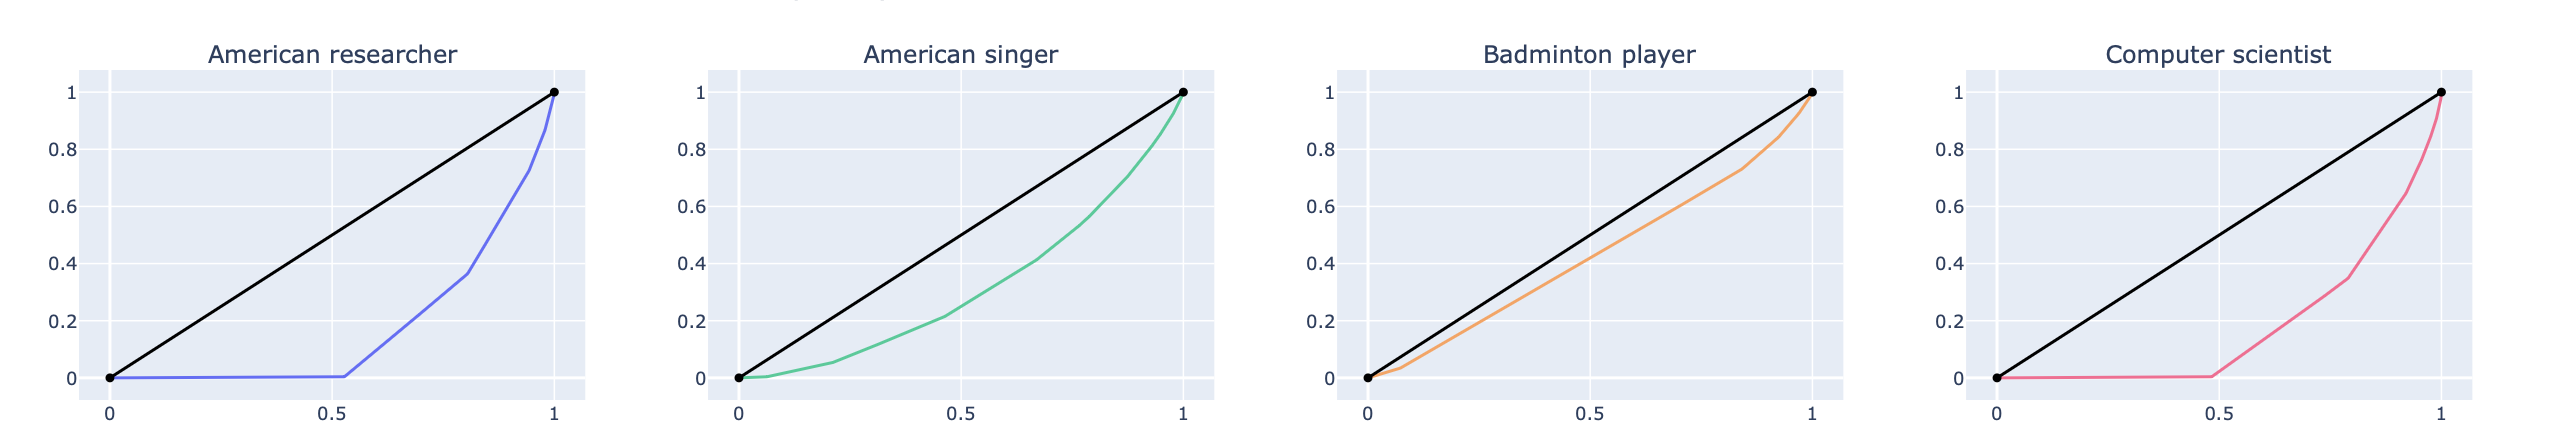
\includegraphics[scale=.5]{Gini - Pure Literal}
    \makebox[\textwidth][c]{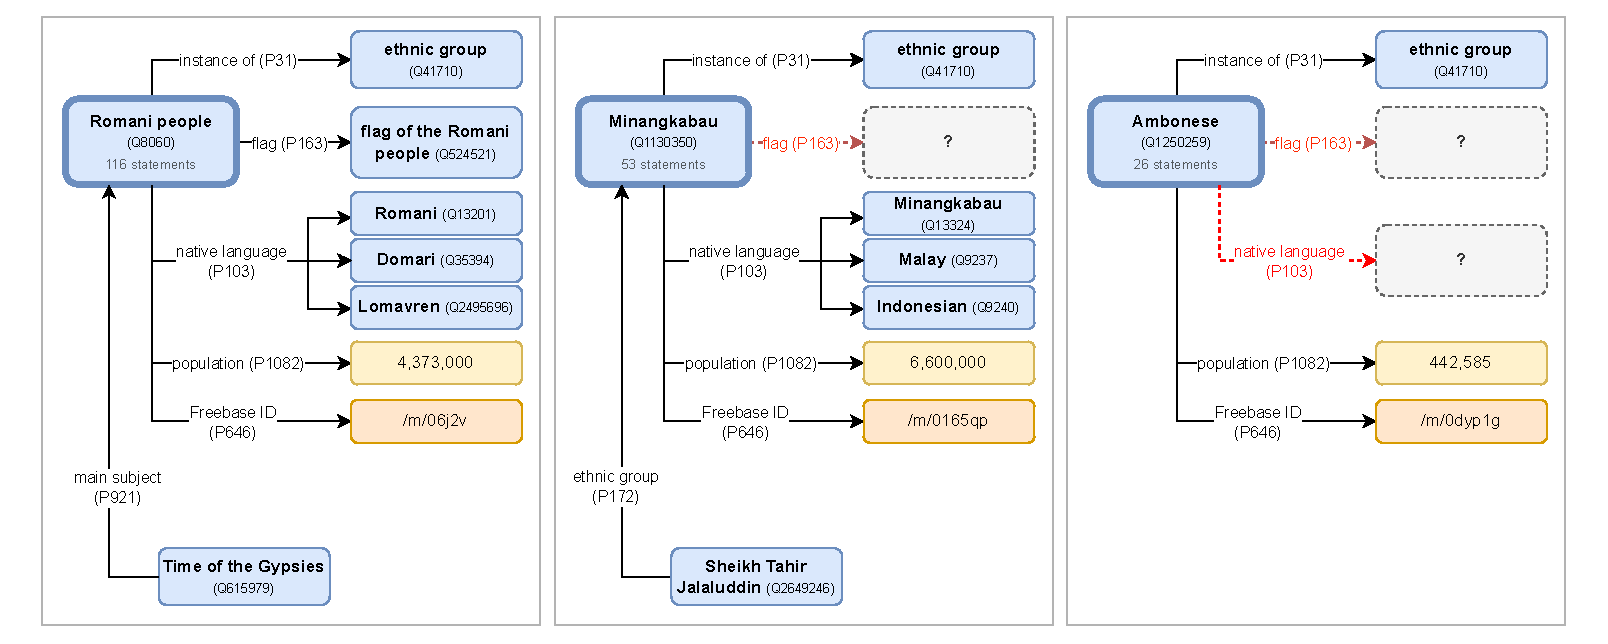
\includegraphics[width=1\textwidth]{Introduction - Wikidata 2}}%
    \caption{Data on Wikidata about the Romani people, the Minangkabau, and the Ambonese retrieved on 17th of February 2025. This figure illustrates how entities of the same class can have variations in their representation, including differences in: \textit{(i)} the properties associated with them, \textit{(ii)} the data types of property values (e.g., objects vs. literals vs. IDs), \textit{(iii)} the cardinality of properties (single vs. multiple values), and \textit{(iv)} the direction of information association (whether entities appear in the subject or object position in RDF triples).} \label{fig:intro-wikidata}
\end{figure}

% Wealth is the abundance of valuable possessions or money, or the state of having this abundance~\cite{wealthOed}. In economics, wealth is defined as the current market value of all assets owned by individuals or households, calculated as total assets minus liabilities~\cite{SaezG16}. When considering individual (human) wealth, the most common measure is net worth. For instance, in Indonesia, wealth reporting for public officials is conducted through the \textit{Laporan Harta Kekayaan Penyelenggara Negara} (LHKPN\footnote{State Official Wealth Report, a mandatory annual report that requires government officials to report their assets to Indonesia's Corruption Eradication Commission (KPK)}), which includes components such as immovable assets (e.g., land and buildings), movable assets (e.g., vehicles), securities, cash and its equivalents, receivables, and liabilities. On the other hand, in knowledge graphs (KGs), wealth can be defined as the amount of information (in terms of properties or links) an entity possesses. Just like the different components of wealth in LHKPN, the wealth of an entity in a KG can be calculated based on different types of properties or links, and with different notion of calculation.

Wealth is the abundance of valuable possessions or money, or the state of having this abundance~\cite{wealthOed}. In economics, wealth is defined as the current market value of all assets owned by individuals or households, calculated as total assets minus liabilities~\cite{SaezG16}. When considering individual (human) wealth, the most common measure is net worth. One important application of this measure is in official asset reporting, where many governments require public officials to disclose their financial for transparency and accountability. For instance, the United States of America mandates government officials and political candidates to submit a public financial disclosure report, while the European Union requires a declaration of interests from its commissioners. In Indonesia, this is done through the \textit{Laporan Harta Kekayaan Penyelenggara Negara\footnote{State Official Wealth Report, a mandatory annual report that requires government officials to report their assets to Indonesia's Corruption Eradication Commission (KPK)}} (LHKPN), which includes components such as immovable assets (e.g., land and buildings), movable assets (e.g., vehicles), securities, cash and its equivalents, receivables, and liabilities.

On the other hand, in knowledge graphs (KGs), wealth can be defined as the amount of information (in terms of properties or links) an entity possesses. Just like the different components of wealth in LHKPN, the wealth of an entity in a KG can be calculated based on different types of properties or links, and with different notion of calculation model. This concept allows us to compare how richly or poorly entities are described within a KG. To illustrate this idea, we examine several entities from Wikidata and the kinds of information they contain.

\autoref{fig:intro-wikidata} shows three Wikidata entities of the type ethnic group: the Romani people, the Minangkabau, and the Ambonese, along with some information about them. For example, the entity Romani people includes information such as its class, flag, native languages, population, and associated Freebase ID. We can observe that a type of information can have a single value, such as the property \textit{flag} for each entity, which is exactly one (or zero, if the information does not exist), or multiple value, such as the property \textit{native language}. Both properties have values that are other Wikidata entities. Additionally, there are other types of properties, such as \textit{population}, which has a static numerical value, and \textit{Freebase ID}, which provides a string used to identify the equivalent entity in the Freebase database.

While the previous examples focus on information with outgoing links, we can also consider the opposite perspective by examining incoming links. This approach does not directly show the possessions of an entity but rather indicates its popularity by showing how often it is mentioned elsewhere, or how other entities declare a sense of ownership or important association with that entity. This is again illustrated by the Romani people being mentioned in \textit{Time of the Gypsies} (through the property \textit{main subject}) and the Minangkabau being associated with Sheikh Tahir Jalaluddin (through the property \textit{ethnic group}).

The example in \autoref{fig:intro-wikidata} provides a clear picture of how entities in Wikidata can have different kinds and amounts of information, which may lead to knowledge imbalance. If this issue is left unaddressed, it can be problematic for anyone utilizing open KGs as a data source. Data users may draw invalid inferences and conclusions based on incomplete or imbalanced data, such as mistakenly assuming that the Minangkabau and Ambonese are less important than the Romani. This imbalance becomes even more striking when considering that the Minangkabau population (6.6 million) is larger than the Romani (4.3 million), yet the Minangkabau entry is less developed, as it is missing basic properties like a flag, and having fewer than half the number of statements (53 vs. 116, as shown in \autoref{fig:intro-wikidata}). If contributors to open KGs cannot identify which entities or classes are lacking information, efforts such as editathons may not be effective, potentially widening the gap between information-rich and information-poor entities. For example, contributors might prioritize enriching the Romani people's data while overlooking gaps in the Minangkabau entry, leaving the \textit{flag} property in the Minangkabau empty despite the well-documented existence of the Marawa flag of Minangkabau which has been existed since 1347\footnote{See the Wikipedia entry on Marawa, the traditional flag of the Minangkabau people: \url{https://id.wikipedia.org/wiki/Marawa}}.

% Existing approaches often focus on ...., lacking a way of quantifying the amount of information contained in KGs. Our study addresses this gap by proposing a formal model to define the knowledge wealth in the RDF knowledge graph. Additionally, we construct an analytical framework using statistical measures and visualization to give insights about the wealth of a class, the inequality between classes, and imbalance measure of wealth within a class. To evaluate this framework, we conducted several use cases on various classes in Wikidata.

% Our contributions are:
% \begin{enumerate}
%     \item We introduce the 3 notions of quantifying knowledge wealth for knowledge graphs, and show how they can be used to further characterize knowledge wealth in knowledge graphs.
%     \item We implemented the formal and insight model using Python programming language and made it accessible.
%     \item We perform a case study on Wikidata classes, showing how biases can be identified in Wikidata, how different definition of wealth impacts the imbalance level of a class, and how the composisition of wealth based on is.
% \end{enumerate}

% Existing approaches often focus on (...), lacking a way of quantifying the amount of information contained in KGs. Our study addresses this gap by proposing a formal model to define the knowledge wealth in the RDF knowledge graph. Specifically, we focus on three key contributions: (i) introducing three notions of quantifying knowledge wealth for knowledge graphs and demonstrating how they can be used to further characterize knowledge wealth; (ii) implementing the formal and insight model using Python and making it accessible for broader use; and (iii) conducting a case study on Wikidata classes, illustrating how biases can be identified, how different definitions of wealth impact the imbalance level of a class, and how the composition of wealth varies between classes.

Existing approaches often focus on enriching knowledge graphs through data population efforts, completeness profiling, or gap detection tools, yet they lack a way of quantifying the amount of information contained in KGs. However, quantification of the amount of information is important to ensure more effective effort in tackling the imbalance and incompleteness issue within KGs. From the previous example, we have already seen the wealth of an entity from three different views: wealth based on the cardinality of property, wealth based on types of property, and wealth based on the direction of link. In addressing the aforementioned gap, our study proposes a knowledge wealth framework to define the knowledge wealth in the RDF knowledge graph. Specifically, we focus on three key contributions: \textit{(i)} introducing three notions of quantifying knowledge wealth for knowledge graphs and demonstrating how they can be used to further characterize knowledge wealth; \textit{(ii)} implementing the formal and insight model as a Python library and making it openly accessible for broader use; and \textit{(iii)} conducting a case study and empirical analysis on Wikidata classes to identify knowledge gaps, highlighting how knowledge wealth varies across gender and regional groups, how different definitions of wealth impact inequality measures, and how structural composition of knowledge wealth across entity classes.

The remainder of this paper is organized into the following sections: Section 2 reviews related work on KG population, data completeness, and knowledge gaps in knowledge graphs; Section 3 introduces the proposed knowledge wealth framework, detailing its formal model, insight model, and Python-based library implementation; Section 4 presents a comprehensive knowledge gap analysis on Wikidata; Section 5 discusses the broader implications of the findings, potential improvements, and future research directions; and Sections 6 concludes the study with a summary of key contributions and outlines opportunities for extending the framework to other knowledge graphs.